\documentclass[presentation]{subfiles}
\onlyinsubfile{}
\setbeamersize{description width=8em}
\begin{document}
\begin{frame}<-3>[label=definitions]{\only<-3>{Before We Get Started\dots}\only<4->{Old Wine in New Bottles}}
  \begin{description}
    \item<1-> [Crowd work] Digitally mediated \alert{information work}, like 
      \emph{image tagging}, \emph{audio transcription}, and \emph{data processing}\par
      \scriptsize{\textcite{crowdworkFuture}\par}\normalsize{}
    \item<2-> [Gig work] Digitally mediated (often \alert{physically embodied}) one--off jobs,
      such as
      \emph{driving for hire},
      \emph{courier services},
      and \emph{administrative support}\par
      \scriptsize{\textcite{friedman2014workers,Parigi:2016:GE:3026779.3013496}\par}\normalsize{}
    \item<3-> [On--demand work] Crowd work and gig work, collectively
  \end{description}
  \visible<5->{
     \begin{center}
        {\color{mLightBrown}
          {\begin{tikzpicture}
            \node  (C) at (0,0) {};
            \node (D) at (9,0) {};
            \path (C) to [ornament=86] (D);
          \end{tikzpicture}}}%
    \end{center}
   }
  \begin{description}
    \item<6-> [\textrm{Piecework}] \textrm{Payment for \emph{output} rather than for \emph{time}}
  \end{description}
\end{frame}


\begin{frame}[standout,label=takeaway]{}
  On--demand work is a modern instantiation of a much older phenomenon
  --- \alert{piecework}.

  {\normalsize The historical arc of piecework
  can shed light on persistent questions
  in this ongoing phenomenon of on--demand work.}
\end{frame}

\againframe<4->{definitions}

\begin{frame}[t]{Payment for \emph{output} rather than for \emph{time}}
  \begin{columns}[T]
    \begin{column}{0.33\textwidth}
      \centering
      Textiles\\
      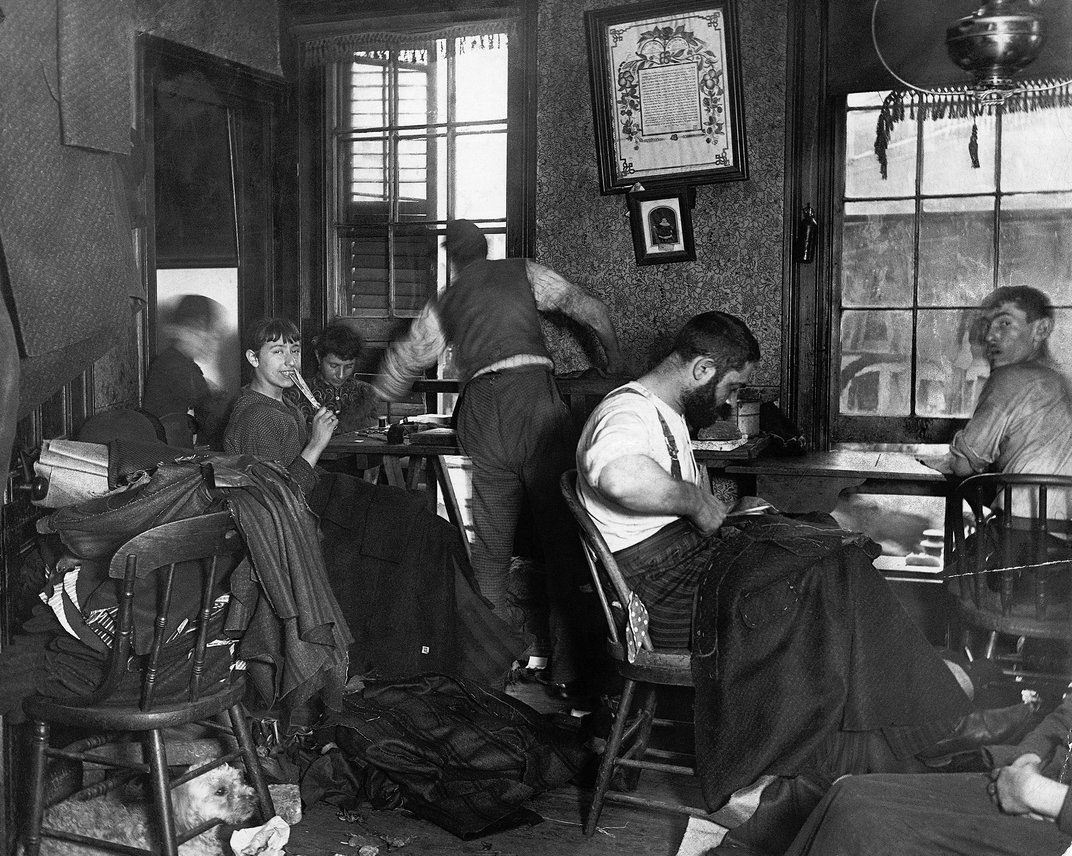
\includegraphics[max width=\linewidth,max height=.3\textheight,keepaspectratio]{figures/pieceworkers.jpg}
    \end{column}
    \begin{column}{0.33\textwidth}
      \centering
      Automobiles\\
      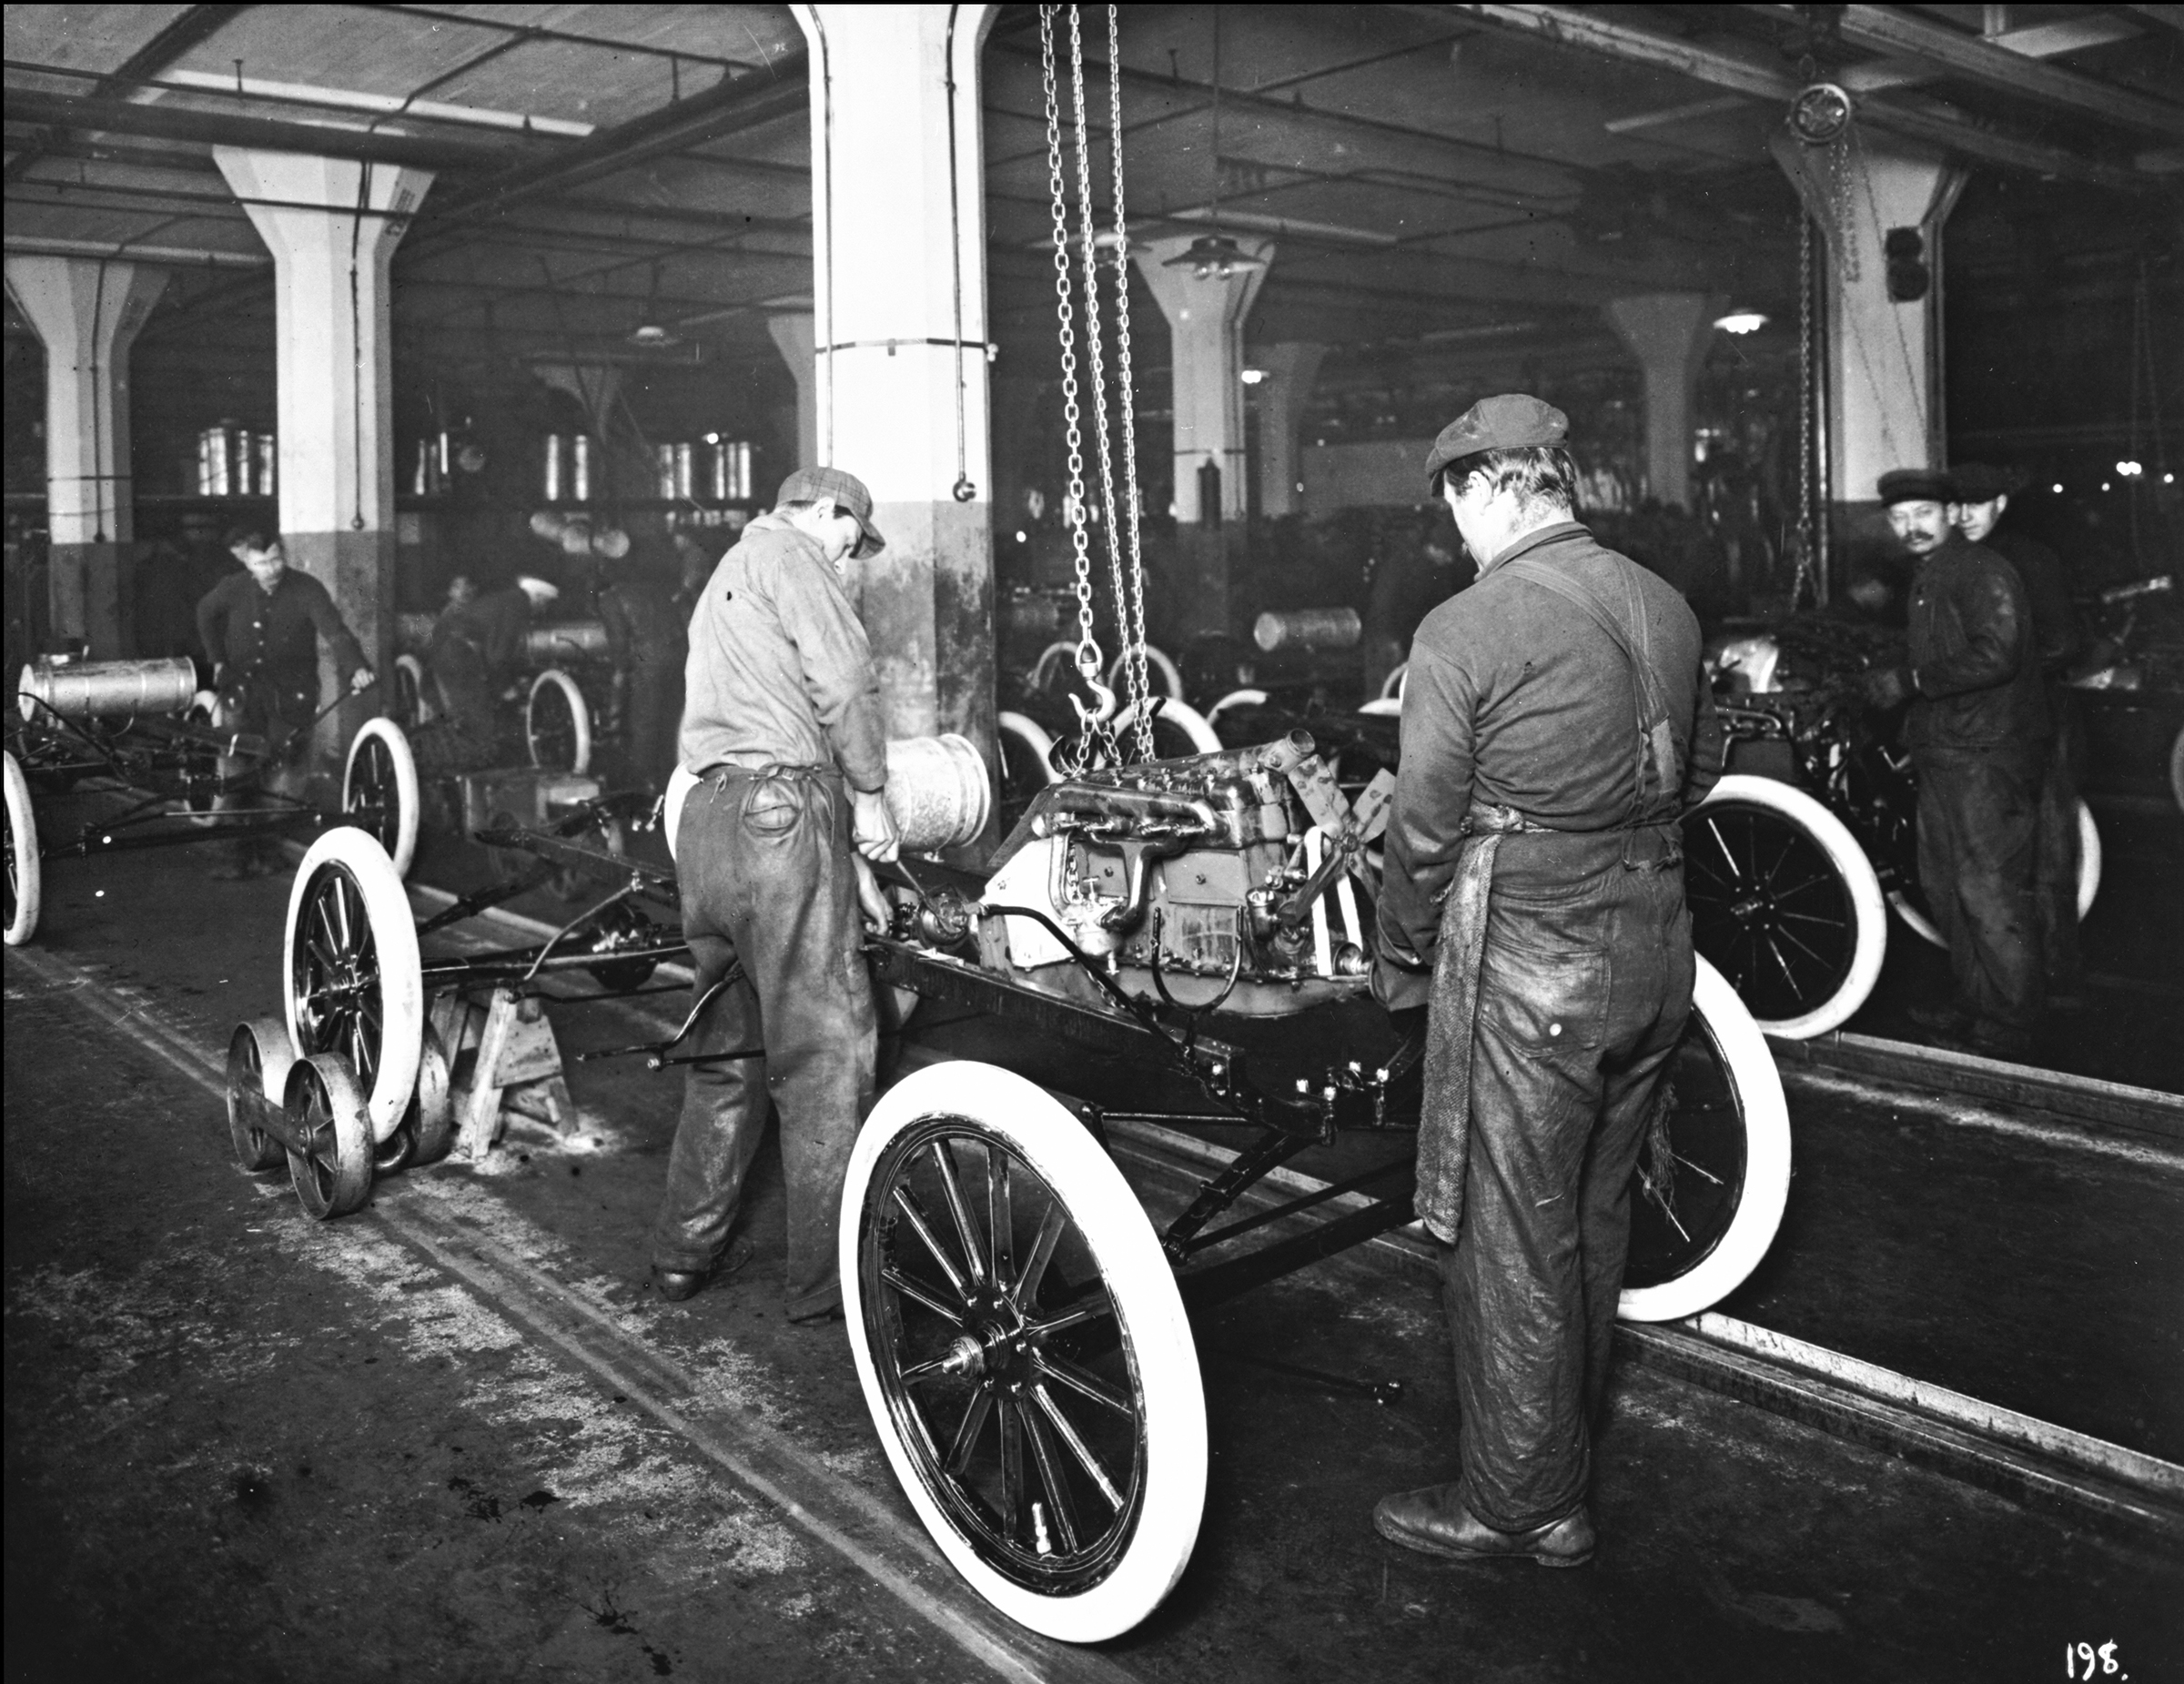
\includegraphics[max width=\linewidth,max height=.3\textheight,keepaspectratio]{figures/photo/ford_assembly_line.jpg}
    \end{column}
    \begin{column}{0.33\textwidth}
      \centering
      Metalwork\\
      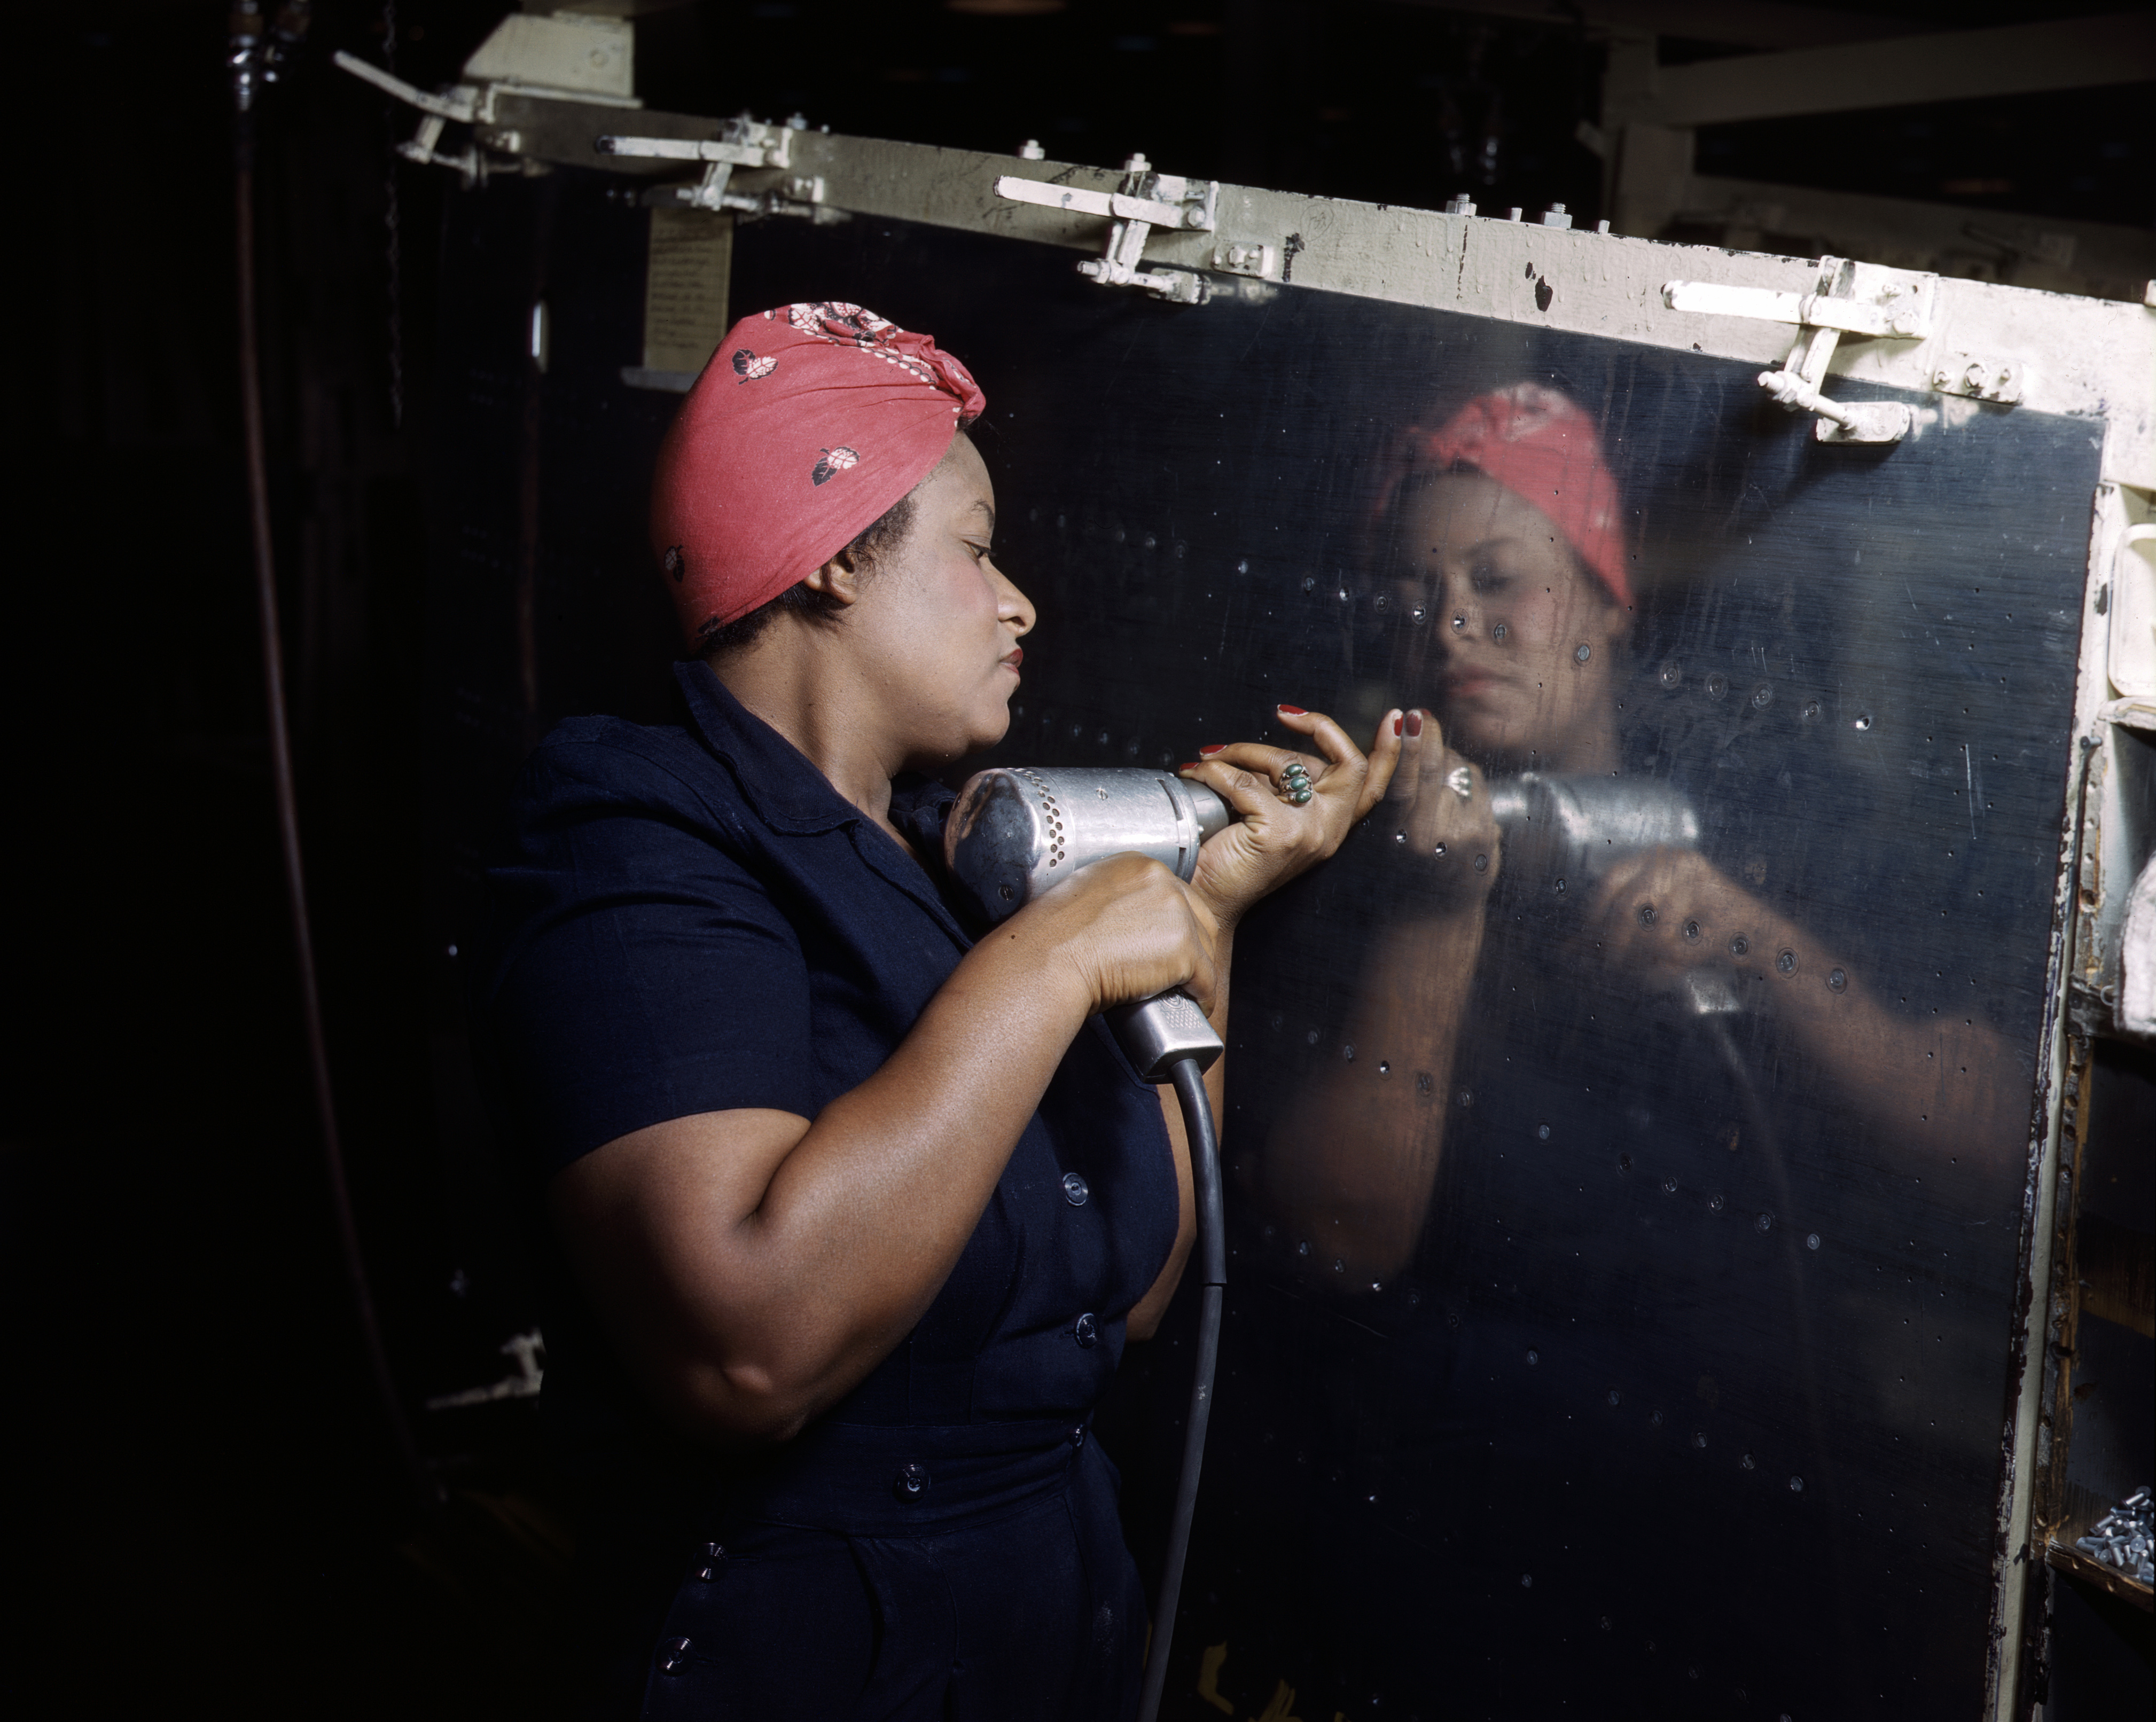
\includegraphics[max width=\linewidth,max height=.3\textheight,keepaspectratio]{figures/photo/Rosie_the_Riveter_(Vultee)_DS.jpg}
    \end{column}
  \end{columns}
  \vspace*{7mm}
  
  \visible<2->{
    \begin{columns}[b]
      \begin{column}[t]{0.45\textwidth}
        \centering
        Crowd work
        \begin{columns}
          \begin{column}[b]{.5\textwidth}
            
\includegraphics[max width=\linewidth,max height=\textheight,keepaspectratio]{figures/amt.png}
          \end{column}
          \begin{column}[b]{.5\textwidth}
            
\includegraphics[max width=\linewidth,max height=\textheight,keepaspectratio]{figures/upwork.png}
          \end{column}
        \end{columns}
      \end{column}

      \begin{column}[t]{0.45\textwidth}
        \centering
        Gig Work
        \begin{columns}
          \begin{column}{.5\textwidth}
            
\includegraphics[max width=\linewidth,max height=\textheight,keepaspectratio]{figures/uber.png}
          \end{column}
          \begin{column}{.5\textwidth}
            
\includegraphics[max width=\linewidth,max height=\textheight,keepaspectratio]{figures/postmates.png}
          \end{column}
        \end{columns}
      \end{column}
    \end{columns}
  }
\end{frame}


\begin{frame}[standout]
    What will be the future of work?
\end{frame}

\begin{frame}{What will be the future of work?}
  \begin{columns}
    \begin{column}{0.6\textwidth}
      \begin{itemize}
        \item<1-> How will \alert{technology} affect the complexity of the work that on--demand workers do?
        \item<2-> What are the \alert{limits} of complexity in on--demand work?
      \end{itemize}
    \end{column}
    \begin{column}{0.4\textwidth}
    \only<3>{
      \centering
      The answers to these questions may predict the \emph{reach} of on--demand work
    }
    \end{column}
    \end{columns}
\end{frame}


\begin{frame}{Thesis}
    This question --- and others like it --- has been asked before.

    History can help us answer them today.

    We'll reach into the history of \alert{piecework}
    --- of human computers, match stick makers, and metalworkers ---
    and show how the \alert{history} of their work can
    inform answers to questions about the \alert{future} of digital work.
\end{frame}

\begin{frame}{Introduction}
  We hope you come away with:
      \begin{itemize}
        \item An \alert{ontological lens} for making sense of on--demand work as a resurgence of piecework
        \item A renewed interest in the use of \alert{historical analysis} to make sense of contemporary phenomena
      \end{itemize}
\end{frame}


\begin{frame}{Comparative Historical Analysis}
  HCI researchers have used historical analysis in the past\par
  \scriptsize{\textcite{Wyche2006,bodker1993historical}\par}\normalsize{}
  
  \dots~But we haven't applied this method to make sense of on--demand work,
        which is a missed opportunity to\dots
  \begin{itemize}
    \item Provide some basic framing for \emph{ostensibly} new phenomena
    \item \emph{Explicate} our theoretical grounding
    \item Flesh out \emph{differences} and their implications
  \end{itemize}
% \end{itemize}
\end{frame}

\notinsubfile{
  \subfile{timeline.tex}
}

\end{document}